\section{Quick Facts}
\subsection{Miscellaneous Tips}
\footnotesize
\blockquote{A DNS server using UDP will query a different authoritative
server if its first query is lost (assuming there are multiple
authoritative servers). It attempts to maximize hit probability.}

\blockquote{A TCP handshake takes 1 RTT}

\blockquote{\textbf{Fast retransmission} requires 3 packets losses to be
triggered, and it halves the cwnd. \textbf{Slow retransmission} waits
for the recovery timer to expire and resets the cwnd}

\blockquote{\textbf{Stub resolver} must know the IP address of a caching
resolver. These are usually are the end users.}

\blockquote{\textbf{Cache resolvers} must know the IP address of a root
server.}

\blockquote{\textbf{Authoritative server} the final source of truth
(either address or CNAME).}

\blockquote{Do not bundle last (optional) ACK and FIN.}

\small
\subsection{Internet Protocol Stack}
\begin{itemize}[itemsep=0em]
  \item \textbf{application}: DNS, FTP, SMTP, HTTP
  \item \textbf{transport}: TCP, UDP
  \item \textbf{network}: IP
  \item \textbf{link}: ethernet, WiFi
\end{itemize}
\subsection{Stateless Protocols}
\begin{itemize}[itemsep=0em]
  \item HTTP/1.1
  \item DNS
  \item UDP
\end{itemize}
\subsection{Stateful Protocols}
\begin{itemize}[itemsep=0em]
  \item TCP
\end{itemize}
\subsection{Has re-trans. timers}
\begin{itemize}[itemsep=0em]
  \item DNS caching resolver
  \item TCP data sender
\end{itemize}
\subsection{DOESN'T have re-trans. Timers}
\begin{itemize}[itemsep=0em]
  \item HTTP client/server
  \item DNS auth. server
  \item TCP data receiver
\end{itemize}
\subsection{Common HTTP responses}
\begin{itemize}[itemsep=0em]
  \item 200 OK: request succeeded
  \item 301 Moved Permanently: object moved to a location specified in the message
  \item 400 bad request: message not understood by server
  \item 505 HTTP version not supported
\end{itemize}
\subsection{Setup UDP (code)}
For client call:
\begin{footnotesize}
  \begin{itemize}[itemsep=-0.5em]
    \item \codebox{socket}
    \item \codebox{recvfrom} and \codebox{sendto} to receive and send data.
  \end{itemize}
\end{footnotesize}
For server call:
\begin{footnotesize}
  \begin{itemize}[itemsep=-0.5em]
    \item \codebox{socket}
    \item \codebox{bind} to an address to use
    \item \codebox{recvfrom} and \codebox{sendto} to receive and send data.
  \end{itemize}
\end{footnotesize}
\subsection{Setup TCP (code)}
For client call:
\begin{footnotesize}
  \begin{itemize}[itemsep=-0.5em]
    \item \codebox{socket}
    \item \codebox{connect} to server through socket
    \item \codebox{recv} and \codebox{send} to receive and send data.
  \end{itemize}
\end{footnotesize}
For server call:
\begin{footnotesize}
  \begin{itemize}[itemsep=-0.5em]
    \item \codebox{socket}
    \item \codebox{bind} to an address to use
    \item \codebox{listen} to mark socket as passive
    \item \codebox{accept} a single client connection
    \item \codebox{recv} and \codebox{send} to receive and send data.
  \end{itemize}
\end{footnotesize}
\subsection{HTTP/1.0}
It uses TCP. Allows 1 request per connection. Each request needs to
reopen a connection. Allows parallel connections. Does not allow
pipelining. Server initiates FIN.
\subsection{HTTP/1.1}
It uses TCP. Connection is persistent. As many requests per connection.
Allows pipelining and parallel connections.
\subsection{HTTP/2.0}
Similar to HTTP/1.1 but it brakes down large packets into frames. This
allows to prevent some forms of head-of-line blocking (cannot prevent
inherent TCP HoL blocking). It also allows to send multiple streams of
data for multiplexing.
\subsection{HTTP Packet Types}
\resizebox{5cm}{!}{
  \begin{tabular}{ |l|l|l|l|l|l|l| }
    \hline
    \multicolumn{1}{|c|}{Type} & \multicolumn{1}{|c|}{HTTP/1.0} & \multicolumn{1}{|c|}{HTTP/1.1} \\
    \hline
    GET    & yes      & yes \\
    \hline
    POST   & yes      & yes \\
    \hline
    HEAD   & yes      & yes \\
    \hline
    PUT    & no       & yes \\
    \hline
    DELETE & no       & yes \\
    \hline
  \end{tabular}
}
\subsection{TCP + TLS}
\begin{center}
  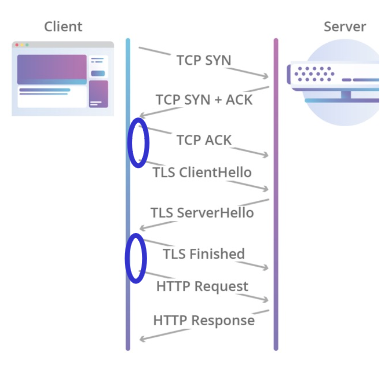
\includegraphics[scale=0.4]{images/tcp-n-tls.png}
\end{center}
\subsection{Stop-and-Wait}
Exactly, that. Stops and waits for the ACK to return before sending the
next packet.
\subsection{Go-Back-N}
Sender has sliding window and can send many unacknowledged packets.
Acknowledgement is for the latest received packet w/o error and sender
window slides. On packet loss it retransmits all packets in the sliding
window. ACKs are cumulative. It does not buffers packets.
\subsection{Selective Repeat}
Sender has sliding window and can send many unacknowledged packets.
Receiver acknowledges each received packet, and it buffers them
(out-of-order if necessary). Sender ``selects'' ACKed packets and
re-sends unACKed ones when their individual timers expire.
\subsection{QUIC}
QUIC does not retransmit a lost packet. Instead it sends it as a later
packet. A QUIC connection has multiple streams which carry frames that
can have multiple types. A frame cannot exeed a packet max size since
they are bundled in a UDP packet.
\subsection{Network Layer}
Uses IP packets. \textbf{Forwarding:} move packets from a router's input
link to appropriate router output link. Trip analogy: process of getting
through single interchange. Data plane, local. \textbf{Routing:}
determine route taken by packets from source to destination. Trip
analogy: process of planning trip from source to destination. Control
plane, network-wide. IP packets have TTL which prevents them from
staying forever in a network (measured in remaining hops).
\subsection{IP Packet Fragmentation}
IP packets are prone to framentation. MTU is used to limite the size of
packets. Packets are only reassembled at destination.
Identifier: generated by the sending host. It identifies all the
segments in the same IP packet and stays unchanged when refragmented.

For flags bit 0 (left most) is reserved, bit 1 (DF bit) prevents
fragmentation if set (dropped if it does not fit), and bit 2 (MF bit)
helps determine the last fragment of a packet (and only the last).

Fragment offset counts from the first byte in the original payload count
in units of 8-byte blocks.
\begin{center}
  \resizebox{5cm}{!}{
  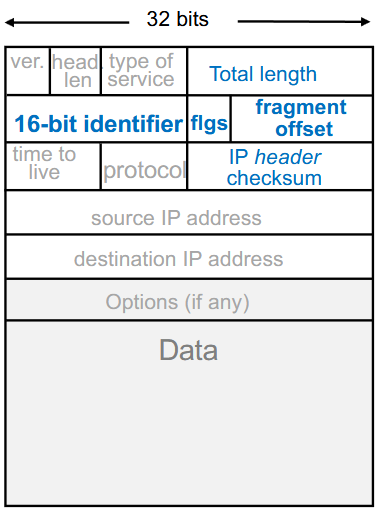
\includegraphics[]{images/ip-frag.png}
  }
\end{center}
\subsection{IP Addressing}
They are delimited with dots and each part is 8 bits. Total has 32 bits.
Common notation for CIDR is \codebox{a.b.c.d/x} where x is the number of
bits dedicated to identify a subnet. The rest are used by router to
identify interfaces within subnet. The complement of x to 32 is the
number of interfaces that the subnet can identify with the caveat that
all 0s and all 1s for subnet are reserved for network address and
broadcast address respectively. Routing favors addresses with larger x
values thus they can have a sort of hierarchy.
\subsection{NAT}
Considered a short-term solution to running out of IPv4 addresses. It
allows a router to map its address plus a port number to an interface
within its subnet. This allows users to freely choose IP addresses
within their subnet rance. They do not have to be unique to those of a
different subnet. Inside is called LAN outside is called WAN. One common
problem is being unable to run services inside a NAT box since that
usually requires to have a specific port number.
\subsection{MAC vs HMAC}
MAC is short piece of information used to authenticate a message. HMAC
is a specific type of MAC that involves a cryptographic hash function
and a secret cryptographic key.
\subsection{Link State Algorithm}
Easiest way is to visually perform Dijkstra while using a priority queue
favoring shortest paths so far. Common notation uses: $D(v)$ pat cost
for current source to destination $v$; $c(x,y)$ link cost from neighbor
$x$ to node $y$; $p(v)$ previous hop from $v$ along best path from
source to $v$ (see table in section \ref{ssec:linkstateexp}). Depends on
global knowledge of network.
\subsection{Distance Vector Algorithm}
Depends only on knowledge of neighbor weights. Uses Bellman-Ford and
neighbor updates to diffuse information.

\remarkbox{
  $D_x(y)=\min\left\{c(x,v) + D_v(y)\right\}$
}

In this equation $v$ represents each neighbor of $x$ and is applied to
each item in a node table. Initially, it is 0 for itself, the respective
cost for neighbors, and infinity for all others. For example, if the
node is $b$ updating its entry for $a$ where $\{a,c,e\}$ are all
neighbor of $b$ then
\begin{scriptsize}
  \remarkbox{
    $D_b(a)=\min\left(c(b,\{a,c,e\}) + D_{\{a,c,e\}}(a)\right)$
  }
\end{scriptsize}
Where $c$ is taken from $b$'s table and $D$ is taken from the neighbors'
tables. Sequence is receive update from neighbors, re-compute, send
updated tables (if anything changed). This can cause something known as
\textit{count to infinity} problem if a suddenly breaks or increases
dramatically in cost. Split horizon and poison reverse mitigate this
issue. The former prevents routing loops by informing neighbors that a
route is unreachable (setting its hop count to infinity) when a router
learns of a failed route, effectively "poisoning" the reverse path.
Failed route can mean that a link cost either increased or completely
failed the immediate neighbors will learn this change and execute poison
reverse.
\subsection{Routing Protocols}
For intra-domain (within) OSPF is used which employs link state to
advertise. For inter-domain (outside) BGP is used and it employs
something similar to distance vector to advertise. Nodes are called
autonomous systems (AS). Intra-AS focuses on performance while inter-AS
puts more emphasis on policy.

For OSPF nodes send HELLO message every 10 seconds. Failure to send for
longer than 40 seconds results in a failure detection. When no failure
occurs for 30 minutes, node sends link-state advertisement (LSA). The
packet contains among other info a TTL, and ID, sequence \#, and list of
direct neighbors and cost of each.

Flooding in OSPF behaves similar to BFS, but if it was parallel and
resolves race conditions with sequence number and visited nodes.
Usually, first arrival.

BGP has two modalities iBGP and eBGP which are BGP sessions between
routers in the same AS and in different AS respectively. When iBGP
favors quickest exit out of network it is called \textit{hot potato}.
Important path attributes include AS-PATH whic is a list of ASes through
which prefix advertisement has passed. NEXT-HOP ndicates specific
internal-AS router to next-hop AS.

BGP route selection in order:
\begin{itemize}[itemsep=0em]
  \item local preference attribute: manually configured value according to AS policies
  \item if same local preference value for multiple routes: choose the one with shortest AS path
  \item then Lowest IGP cost (hot potato routing)
\end{itemize}
\subsection{Ethernet CSMA/CD Algorithm}
(1) NIC receives datagram from network layer, creates frame. (2) If NIC
senses channel idle, starts frame transmission. If NIC senses channel
busy, waits until channel idle, then transmits ``1-persistent''. (3) If
NIC transmits entire frame without detecting another transmission, NIC
is done with frame! (4) If NIC detects another transmission while
transmitting, aborts and sends \textbf{jam signal} for a short time
period. (5) After aborting, NIC enters binary exponential backoff: after
mth collision, NIC chooses a value K at random from ${0,1,2,\dots, 2m -
1}$. Then NIC waits K slots, returns to Step 2. One slot available means
transmission time for 512 bits; otherwise, more collisions means much
longer backoff interval.
\subsection{Link Layer Data Framing}
Blocks of data are called differently for different layers: frame at
link layer, datagram at network layer, and segment at transport layer. A
frame has a header field and optionally it may have a trailer field
after the data. Byte-Oriented Framing Protocol: delineate frame with a
byte of special bit sequence: 01111110. If the bit sequence 01111110
occurs in data stream, sender adds (“stuffs”) extra 01111110 byte after
each appearance of 01111110 (see section \ref{ssec:bytestuffing}).